\chapter{Hardware Design and Implementation}
\label{ch:hardware}

The power PCB combines the charge-pump resonant circuit from earlier DTU work and planar magnetics with the input network, auxiliary supplies, isolated feedback, USB-C output stage, and digital control developed in this project. The MCU acquires primary voltage, secondary-bulk voltage, and half-bridge current at PA0--PA2. On the original prototype, carrier commands at PA8/PA9 and burst enable at PA10 control energy transfer. The V2 assignments are given in \cref{sec:hw-v2}.

Bring-up required corrections to the timer connections and changes to the resonant branch. The V2 schematic excerpts show the common power circuit; fitted components and controller assignments are identified for each tested board. The following sections describe the tested assembly, later circuit revisions, and V3 layout.

\section{Prototype and Board Revisions}
\label{sec:hw-overview}

One V1.0 PCB was assembled for bring-up and the final tests. It measures \SI{202.77}{\milli\metre} by \SI{72.77}{\milli\metre} and has four 1~oz copper layers. The final resonant branch had two Wurth Elektronik 7443640470B inductors connected in series. The voltage-control firmware used for the final tests is described in Chapter~\ref{ch:control}.

Changes made during bring-up were recorded in V1.1. The timer-pin assignment and charge-pump-diode connection were corrected. Some component values and positions were also changed. No separate V1.1 board was manufactured. Differences between the drawings and fitted parts are noted so the tested configuration can be reproduced. Both complete schematic revisions are included in Appendix~\ref{app:hardware}.

\begin{table}[htbp]
\centering
\caption{Hardware used for the prototype tests.}
\label{tab:hardware-revision-status}
\begin{tabularx}{\textwidth}{@{}p{0.19\textwidth}p{0.31\textwidth}X@{}}
\toprule
Hardware & Build status & Use\\
\midrule
V1.0 board & Manufactured and tested, including bring-up modifications & Board shown in the photographs, layout, and measurements\\
Final resonant branch & Two \SI{4.7}{\micro\henry} resonant inductors in series & Used for the final tests\\
V1.1 schematic & Drawing revision; no separate test board & Documents the bring-up corrections\\
\bottomrule
\end{tabularx}
\end{table}

V2 continued this work with the MCU integrated on the converter board. The schematic and four-layer PCB layout are described in \cref{sec:hw-v2}. Preliminary powered V2 tests, including the leakage-only tank change and remaining input-bridge heating, are described in \cref{sec:res-v2-testing}. The earlier matched measurements were taken on the modified V1.0 board.

Before fabrication, the board passed the configured Altium design-rule check. During bring-up, insulation was checked at \SI{1000}{\volt} for \SI{30}{\second} with the available handheld tester. This was a laboratory check; standardized safety qualification requires a defined test procedure and conditions.

\begin{figure}[H]
\centering
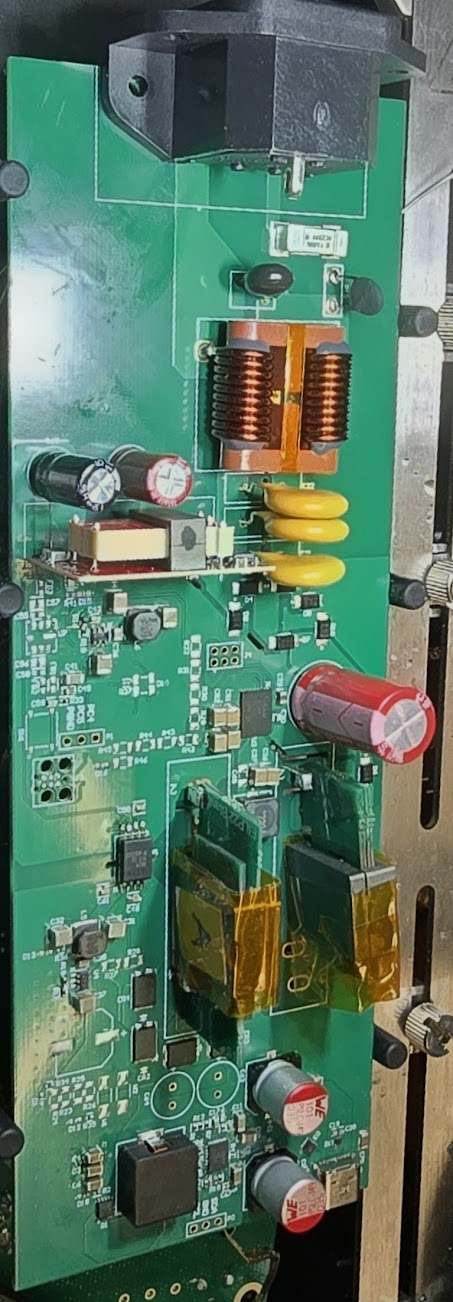
\includegraphics[angle=90,width=\linewidth]{Pictures/Thesis/07_Hardware/final_prototype_main_photo.png}
\caption{Assembled V1.0 prototype used for the final tests.}
\label{fig:final-prototype-main-photo}
\end{figure}

\section{Input Protection, Filtering, and Rectification}
\label{sec:hw-input}

The AC input passes through the connector, fuse, inrush element, varistor, filter, and bridge. The rectified line then supplies the charge pump. The input side includes a capacitor-discharge circuit. The filter connections also carry high-frequency return current from the switching stage and were treated as part of the power loop.

The input fuse is a Littelfuse 04653.15DR rated at \SI{3.15}{\ampere} and \SI{250}{\volt} AC \cite{littelfuse0465315dr}. A Panasonic ERZV07D471 clamps surges \cite{panasonicERZV07D471}. The V1.0 component list specifies a Wurth Elektronik 7448680200 common-mode choke with two \SI{120}{\micro\henry} windings \cite{wurth7448680200}. V1.1 shows a single \SI{100}{\micro\henry} 7447480101 element at L2 instead. This change was made in the drawing; a second filter assembly was not tested.

\begin{figure}[htbp]
\centering
\begin{subfigure}[t]{0.97\textwidth}
\centering
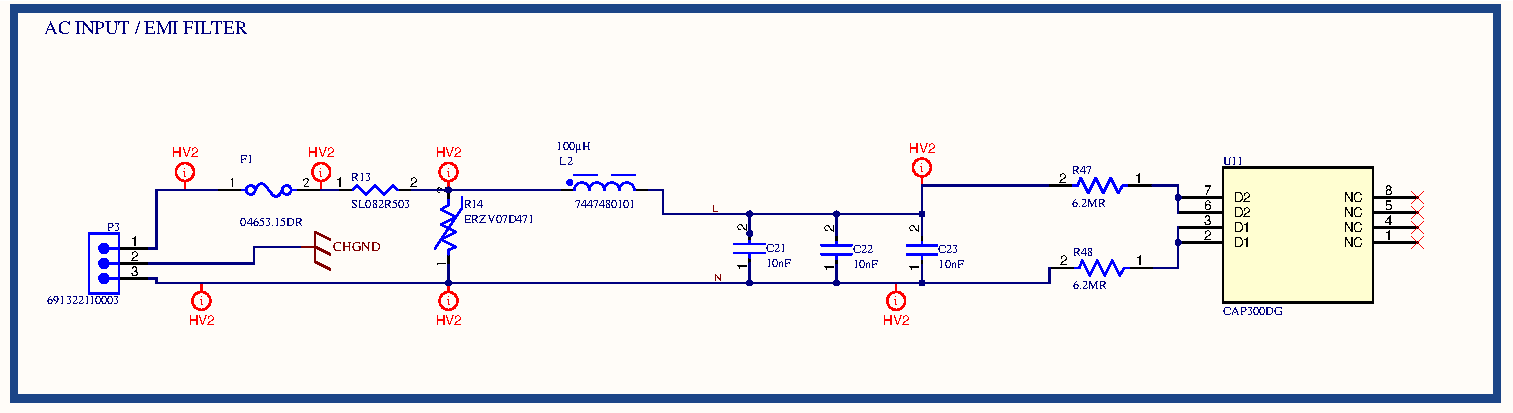
\includegraphics[page=1,width=\textwidth]{Pictures/Thesis/07_Hardware/Rebuilt/schematic_v2_input_excerpt.pdf}
\caption{Input connector, fuse, inrush element, varistor, filter, and discharge circuit.}
\end{subfigure}
\par\medskip
\begin{subfigure}[t]{0.38\textwidth}
\centering
\includegraphics[page=2,width=\textwidth]{Pictures/Thesis/07_Hardware/Rebuilt/schematic_v2_input_excerpt.pdf}
\caption{Bridge rectifier.}
\end{subfigure}
\caption{V2 sheet 3 input filter and full-bridge rectifier.}
\label{fig:hw-input-schematic}
\end{figure}

Bridge commutation, diode capacitance, charge-pump current, and loop inductance couple this path to the half bridge. The assembly's input behavior was assessed from the input-current measurements in Chapter~\ref{ch:results}; measurements on both sides of the installed filter are still needed to determine its noise attenuation.

\section{High-Frequency Power Stage}
\label{sec:hw-powerstage}
\subsection{Charge-Pump Branch and DC Link}
\label{sec:hw-pump}

The charge-pump branch connects the rectified line to VSW and the high-voltage DC link. In the V2 drawing, C24 is the \SI{2}{\nano\farad} pump capacitor, L3 is the pump-path inductance, and D6--D8 steer charge into the link. The isolated resonant path also starts at VSW, so the same half bridge drives input-current shaping and power transfer.

A KEMET C1206X202FBGACTU pump capacitor was used, rated \SI{2000}{\pico\farad}, \SI{630}{\volt}, \(\pm1\%\), C0G/NP0 \cite{kemetC1206X202FBGACTU}. Its capacitance sets the charge moved in each cycle. The component list specifies PU1JLWH \SI{600}{\volt}, \SI{1}{\ampere} ultrafast pump rectifiers \cite{taiwansemiPU1JLWH} and a Wurth Elektronik 860241478004 \SI{22}{\micro\farad}, \SI{450}{\volt} DC-link capacitor \cite{wurth860241478004}. C25 is specified as \SI{22}{\micro\farad} in V1.0 and \SI{10}{\micro\farad} in V1.1. The component list and V1.0 board value describe the tested link.

The branch carries pulsed current as the line voltage changes. The operating margin still needs to be checked by measuring peak and RMS diode current, capacitor current, DC-link ripple and peak voltage, and loop overshoot. The results can then be compared with the part ratings.

\begin{landscape}
\begin{figure}[htbp]
\centering
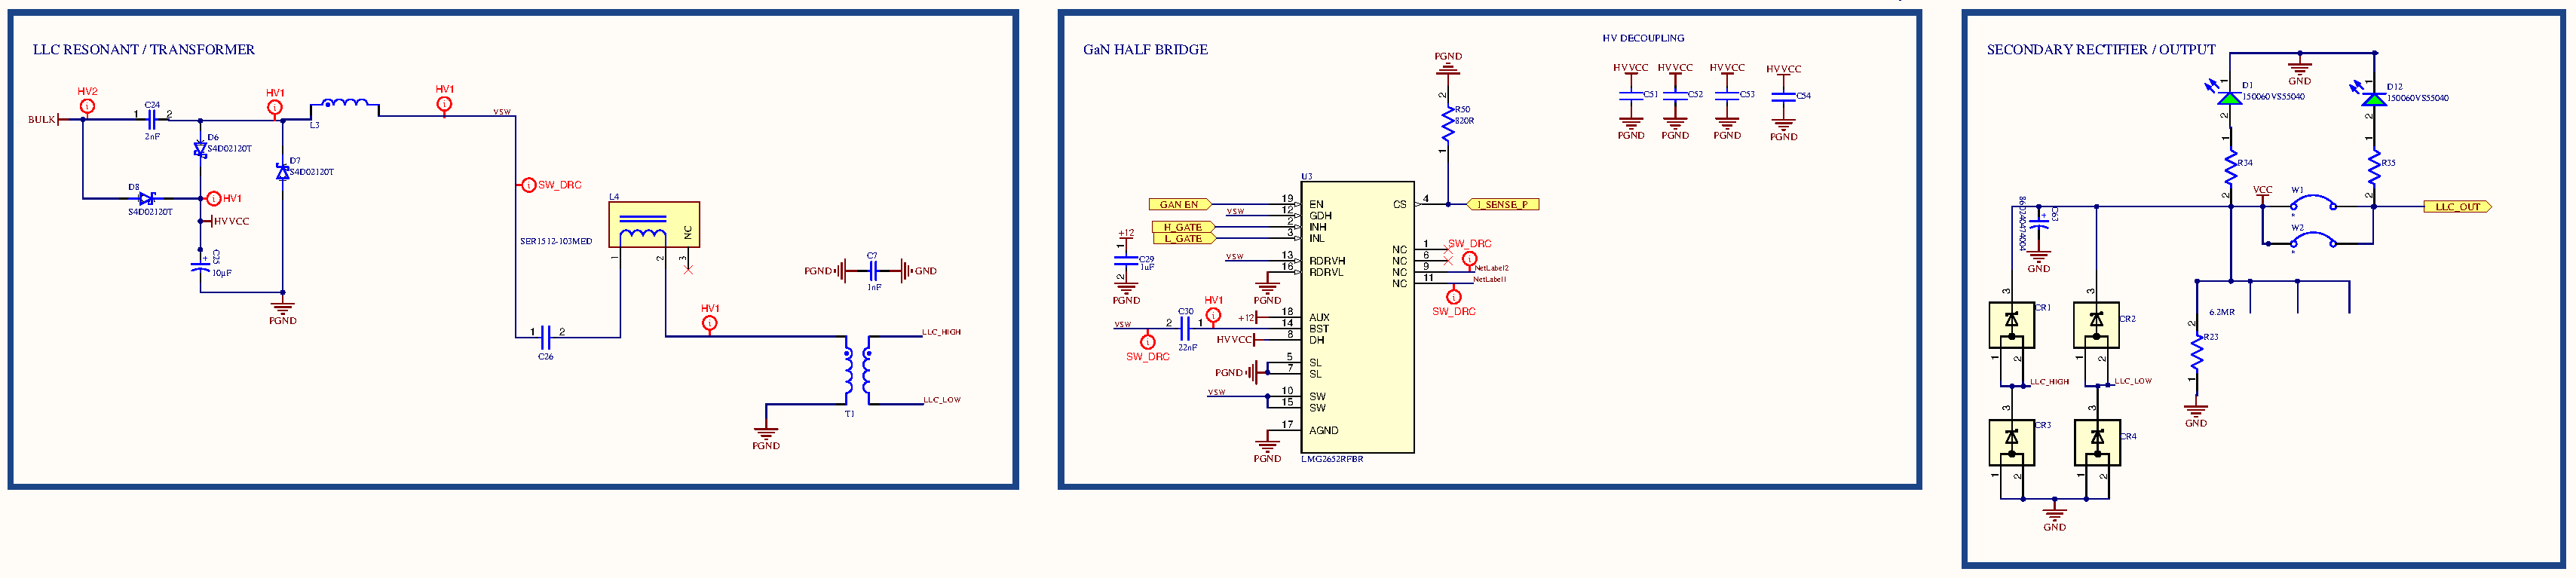
\includegraphics[width=0.98\linewidth,height=0.77\textheight,keepaspectratio]{Pictures/Thesis/07_Hardware/Rebuilt/schematic_v2_power_stage_excerpt.pdf}
\caption{V2 sheet 3 charge-pump and resonant power circuit. C24 and D6--D8 form the pump branch, the GaN half bridge drives the tank and transformer, and the secondary bridge supplies the isolated bulk output.}
\label{fig:schematic-power-stage}
\end{figure}
\end{landscape}

\subsection{Integrated GaN Half Bridge}
\label{sec:hw-halfbridge}

The shared switching stage uses the LMG2652RFBR, which integrates two \SI{650}{\volt} GaN FETs, gate drivers, high-side level shifting, bootstrap support, current-sense emulation, and protection in an \SI{8}{\milli\metre} by \SI{6}{\milli\metre} package \cite{tiLMG2652}. Integration reduces external gate-drive connections, but local bias decoupling, short commutation loops, controlled switch-node area, and PCB heat spreading remain necessary.

\begin{table}[htbp]
\centering
\caption{LMG2652 ratings and characteristics \cite{tiLMG2652}, under the data-sheet test conditions.}
\label{tab:lmg2652-ratings}
\small
\begin{tabularx}{\textwidth}{@{}p{0.29\textwidth}p{0.31\textwidth}X@{}}
\toprule
Parameter & Value & Design consideration\\
\midrule
FET voltage rating & \SI{650}{\volt} & Compare with DC-link voltage plus overshoot.\\
Typical on-resistance & \SI{140}{\milli\ohm} at \SI{25}{\celsius}; \SI{255}{\milli\ohm} at \SI{125}{\celsius} & Conduction loss increases with temperature.\\
Bias and bootstrap rails & AUX \SIrange{10}{26}{\volt}; BST--SW \SIrange{7.5}{26}{\volt} & Verify rail and bootstrap behavior before switching.\\
Recommended capacitance & \(C_{\mathrm{BST}}\geq\SI{10}{\nano\farad}\), \(C_{\mathrm{AUX}}\geq3C_{\mathrm{BST}}\) & Account for capacitance under operating bias.\\
Recommended continuous drain current & \(\pm\SI{6.1}{\ampere}\) per FET & Check current and temperature together.\\
Output-capacitance quantities & \(Q_{\mathrm{OSS}}=\SI{21.8}{\nano\coulomb}\), \(C_{\mathrm{OSS}}=\SI{34.2}{\pico\farad}\), \(E_{\mathrm{OSS}}=\SI{3.0}{\micro\joule}\) & Allow enough commutation current to charge and discharge the output capacitances.\\
Reverse-recovery charge & \(Q_{\mathrm{RR}}=\SI{0}{\nano\coulomb}\) & GaN commutation differs from a silicon body diode.\\
Cycle-by-cycle current limit & \SIrange{5.6}{7.4}{\ampere}; \SI{6.5}{\ampere} typical & This device limit is separate from PA2 firmware thresholds.\\
Overtemperature trip/reset & \SI{165}{\celsius}/\SI{150}{\celsius} & Protection thresholds are not a normal operating target.\\
Junction range and thermal metrics & \SIrange{-40}{150}{\celsius}; \(R_{\theta JA}=\SI{22.7}{\celsius\per\watt}\), \(R_{\theta JC(\mathrm{bot})}=\SI{1.20}{\celsius\per\watt}\) & These values depend on the specified mounting and cooling conditions.\\
\bottomrule
\end{tabularx}
\end{table}

The driver delays are comparable to the programmed dead time. At the data-sheet condition of \SI{400}{\volt} and \SI{1.8}{\ampere}, low-side turn-on/turn-off delays are \SI{40}{\nano\second}/\SI{45}{\nano\second}. High-side turn-on is \SI{45}{\nano\second} from INH or \SI{40}{\nano\second} from GDH, while turn-off is \SI{55}{\nano\second} or \SI{45}{\nano\second}, respectively. The listed turn-on slew rate is \SI{80}{\volt\per\nano\second} \cite{tiLMG2652}. These delays affect the switch-node timing. Actual transistor dead time must be measured; timer settings alone are insufficient.

The half-bridge switch node, labeled VSW, also couples through capacitance to neighboring copper, the transformer, and the probes. Both device switching and the installed loop contribute to ringing. Soft turn-on must be checked from the incoming switch's voltage and current at the stated input and load, using the probing method in \cref{sec:method-probing}.

\subsection{Logic Commands and Dead Time}
\label{sec:hw-gatedrive}

On the original prototype, center-aligned TIM1 generates the fixed \SI{1}{\mega\hertz} carrier on MCU pins PA8/PA9. The separate burst-enable output at PA10 drives the integrated driver's EN input, adjusting average transfer without changing carrier frequency. A dead interval is programmed at both carrier transitions to prevent simultaneous switch commands.

The original V1.0 pin assignment did not provide the intended carrier pair. The PA8/PA9/PA10 correction was recorded in V1.1, with a nominal \SI{40}{\nano\second} interval used during development. The available switch-node traces show switching behavior, but matched gate-timing and commutation-current captures are needed to measure effective dead time and check ZVS over the input and load range.

\subsection{Resonant Path, Transformer, and Rectifier}
\label{sec:hw-output}

The transformer primary is connected to VSW through the resonant capacitor and added series inductance. CR1--CR4 rectify the secondary energy into a bulk supply for the MPQ4242 output stage. The USB-C PD stage regulates the output voltage from this bulk supply.

Several inductor arrangements were tried during bring-up. The final assembly has two Wurth Elektronik 7443640470B inductors connected in series, each nominally \SI{4.7}{\micro\henry}. Together they add \SI{9.4}{\micro\henry}, with an individual tolerance of \(\pm20\%\). Each has a maximum DC resistance of \SI{0.97}{\milli\ohm} at \SI{20}{\celsius}, giving \SI{1.94}{\milli\ohm} for the pair before the connecting wires \cite{wurth7443640470b}. Both parts carry the same current. Loss is spread across the two packages, but either part's temperature can still limit operation.

With approximately \SI{16.5}{\micro\henry} transformer leakage and the \SI{1}{\nano\farad} capacitor, the first-order resonance lies near the \SI{1}{\mega\hertz} carrier. That estimate depends on the fitted transformer, component tolerances, and connecting conductors, as explained in \cref{sec:analysis-resonant,sec:mag-parasitics}. The L4 value in V1.1 does not represent this final series pair.

\begin{figure}[H]
\centering
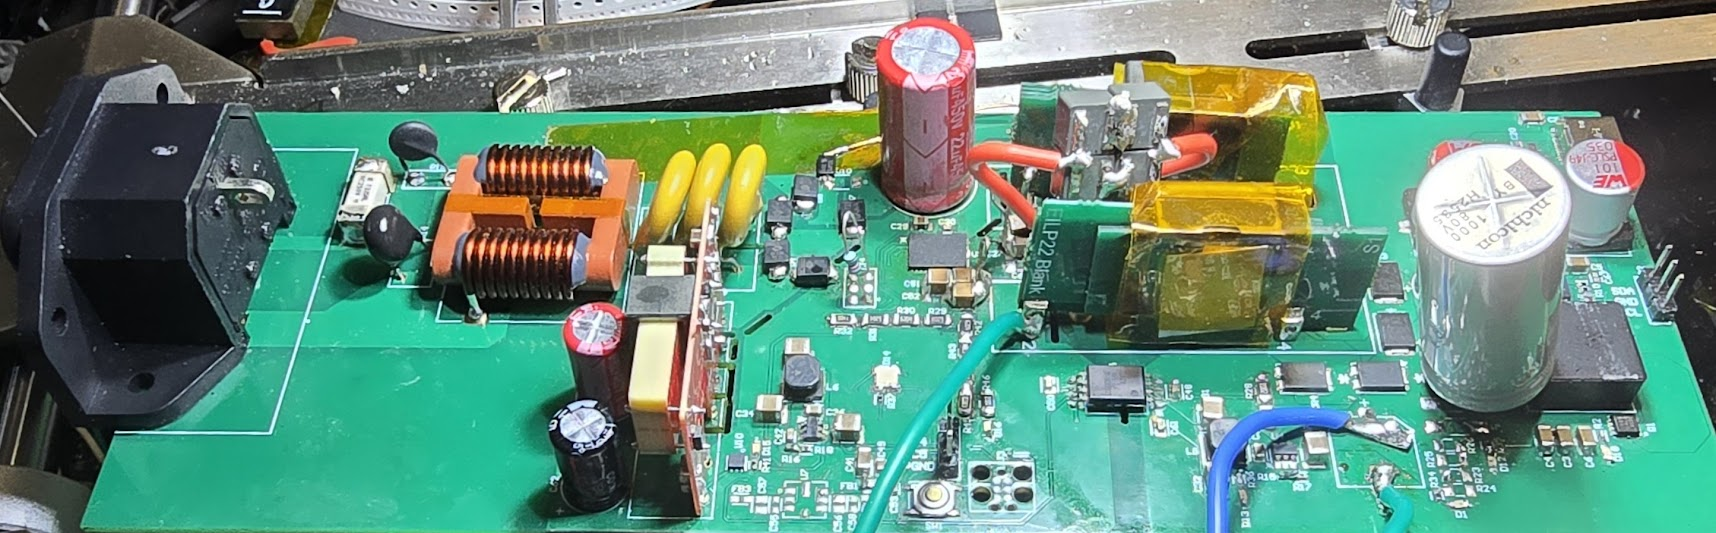
\includegraphics[width=\textwidth,height=0.35\textheight,keepaspectratio]{Pictures/Thesis/07_Hardware/resonant_inductor_test_variants.png}
\caption{Resonant-inductor arrangements tested during bring-up.}
\label{fig:resonant-inductor-test-variants}
\end{figure}

\begin{figure}[H]
\centering
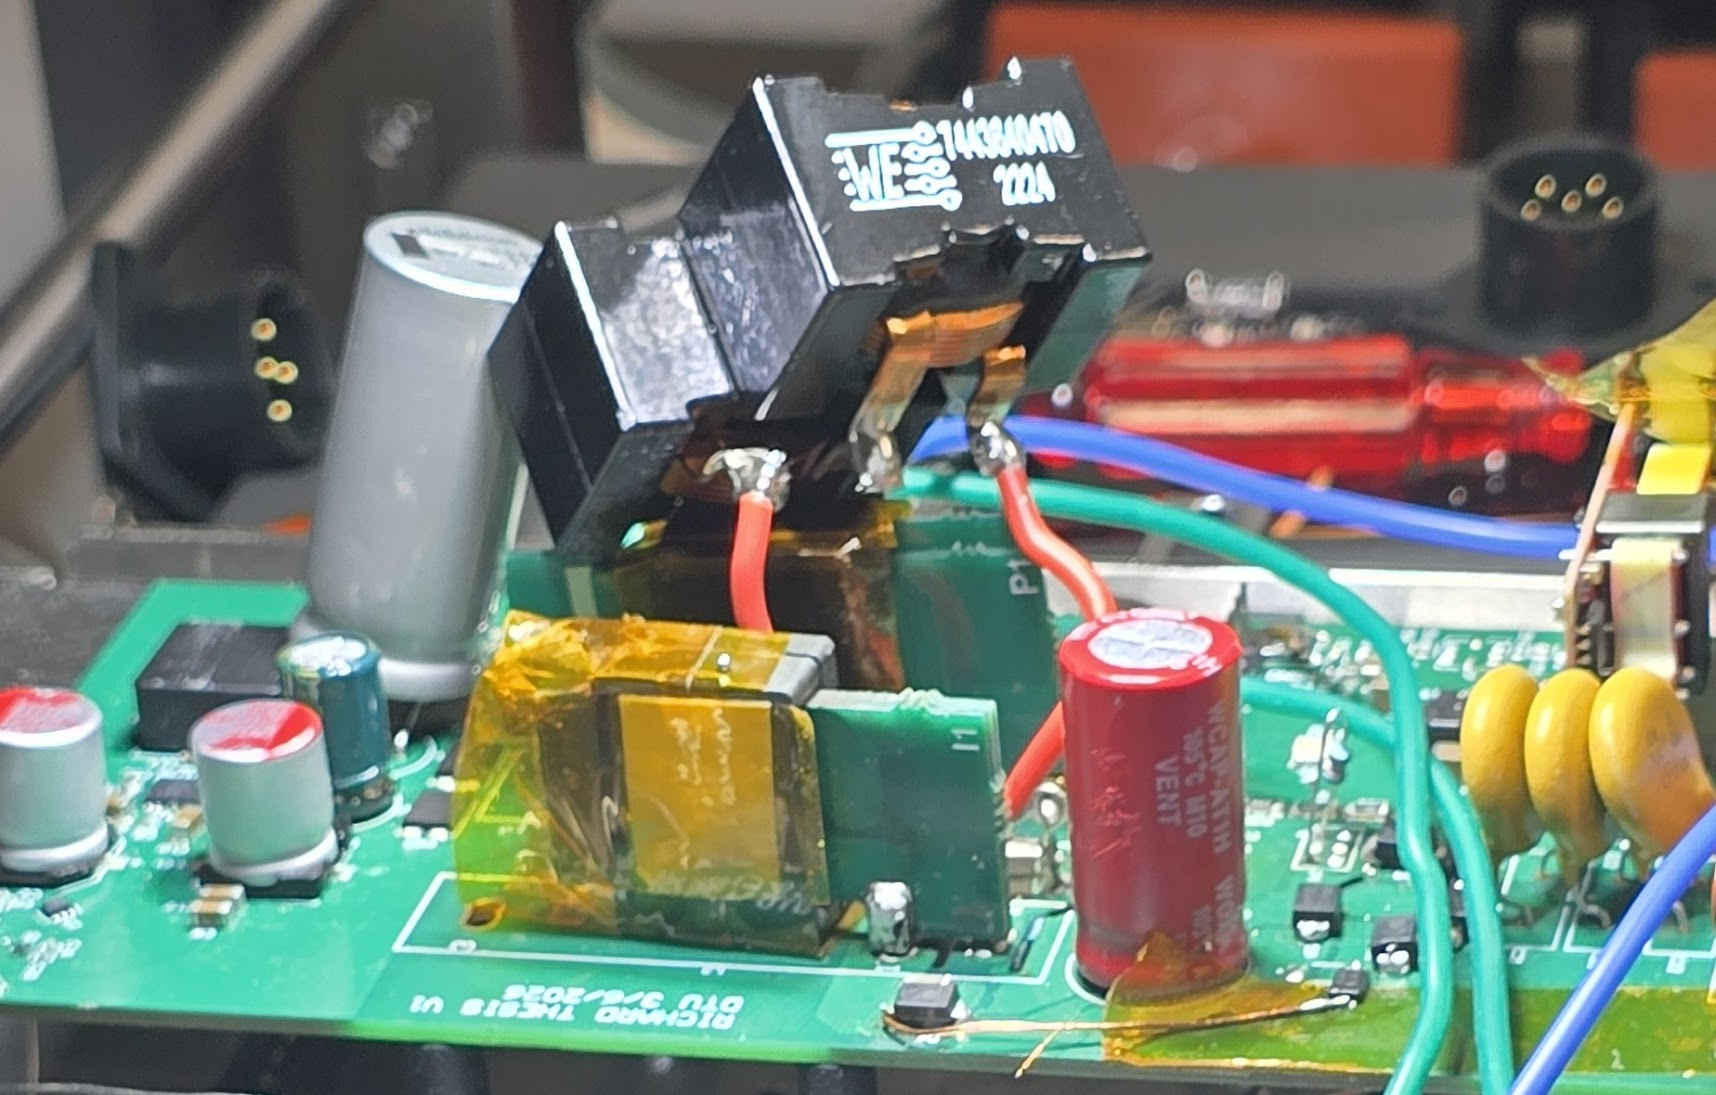
\includegraphics[width=\textwidth,height=0.35\textheight,keepaspectratio]{Pictures/Thesis/07_Hardware/final_resonant_inductor_usb_pdo.png}
\caption{Final series-inductor configuration and output-test arrangement.}
\label{fig:final-resonant-inductor-usb-pdo}
\end{figure}

Changing the resonant branch affects tank current, gain, and the charge available to change VSW during commutation. Waveform comparisons therefore need the fitted inductor arrangement. The installed path must be measured before the model is used to select another change.

\section{USB-C Output Stage}
\label{sec:hw-usbc}

The MPQ4242GVE-0000-AEC1-P stage regulates the USB-C output voltage from the isolated bulk supply. The stage includes the switching inductor, output power path, current-sense element, bulk and ceramic capacitors, CC connections, data-line protection, and VBUS TVS protection. In \Cref{fig:schematic-usbc}, \texttt{V\_PW\_OUTPUT\_BULK} feeds the stage and \texttt{USB\_PD\_OUT} supplies the USB-C output.

\begin{landscape}
\begin{figure}[htbp]
\centering
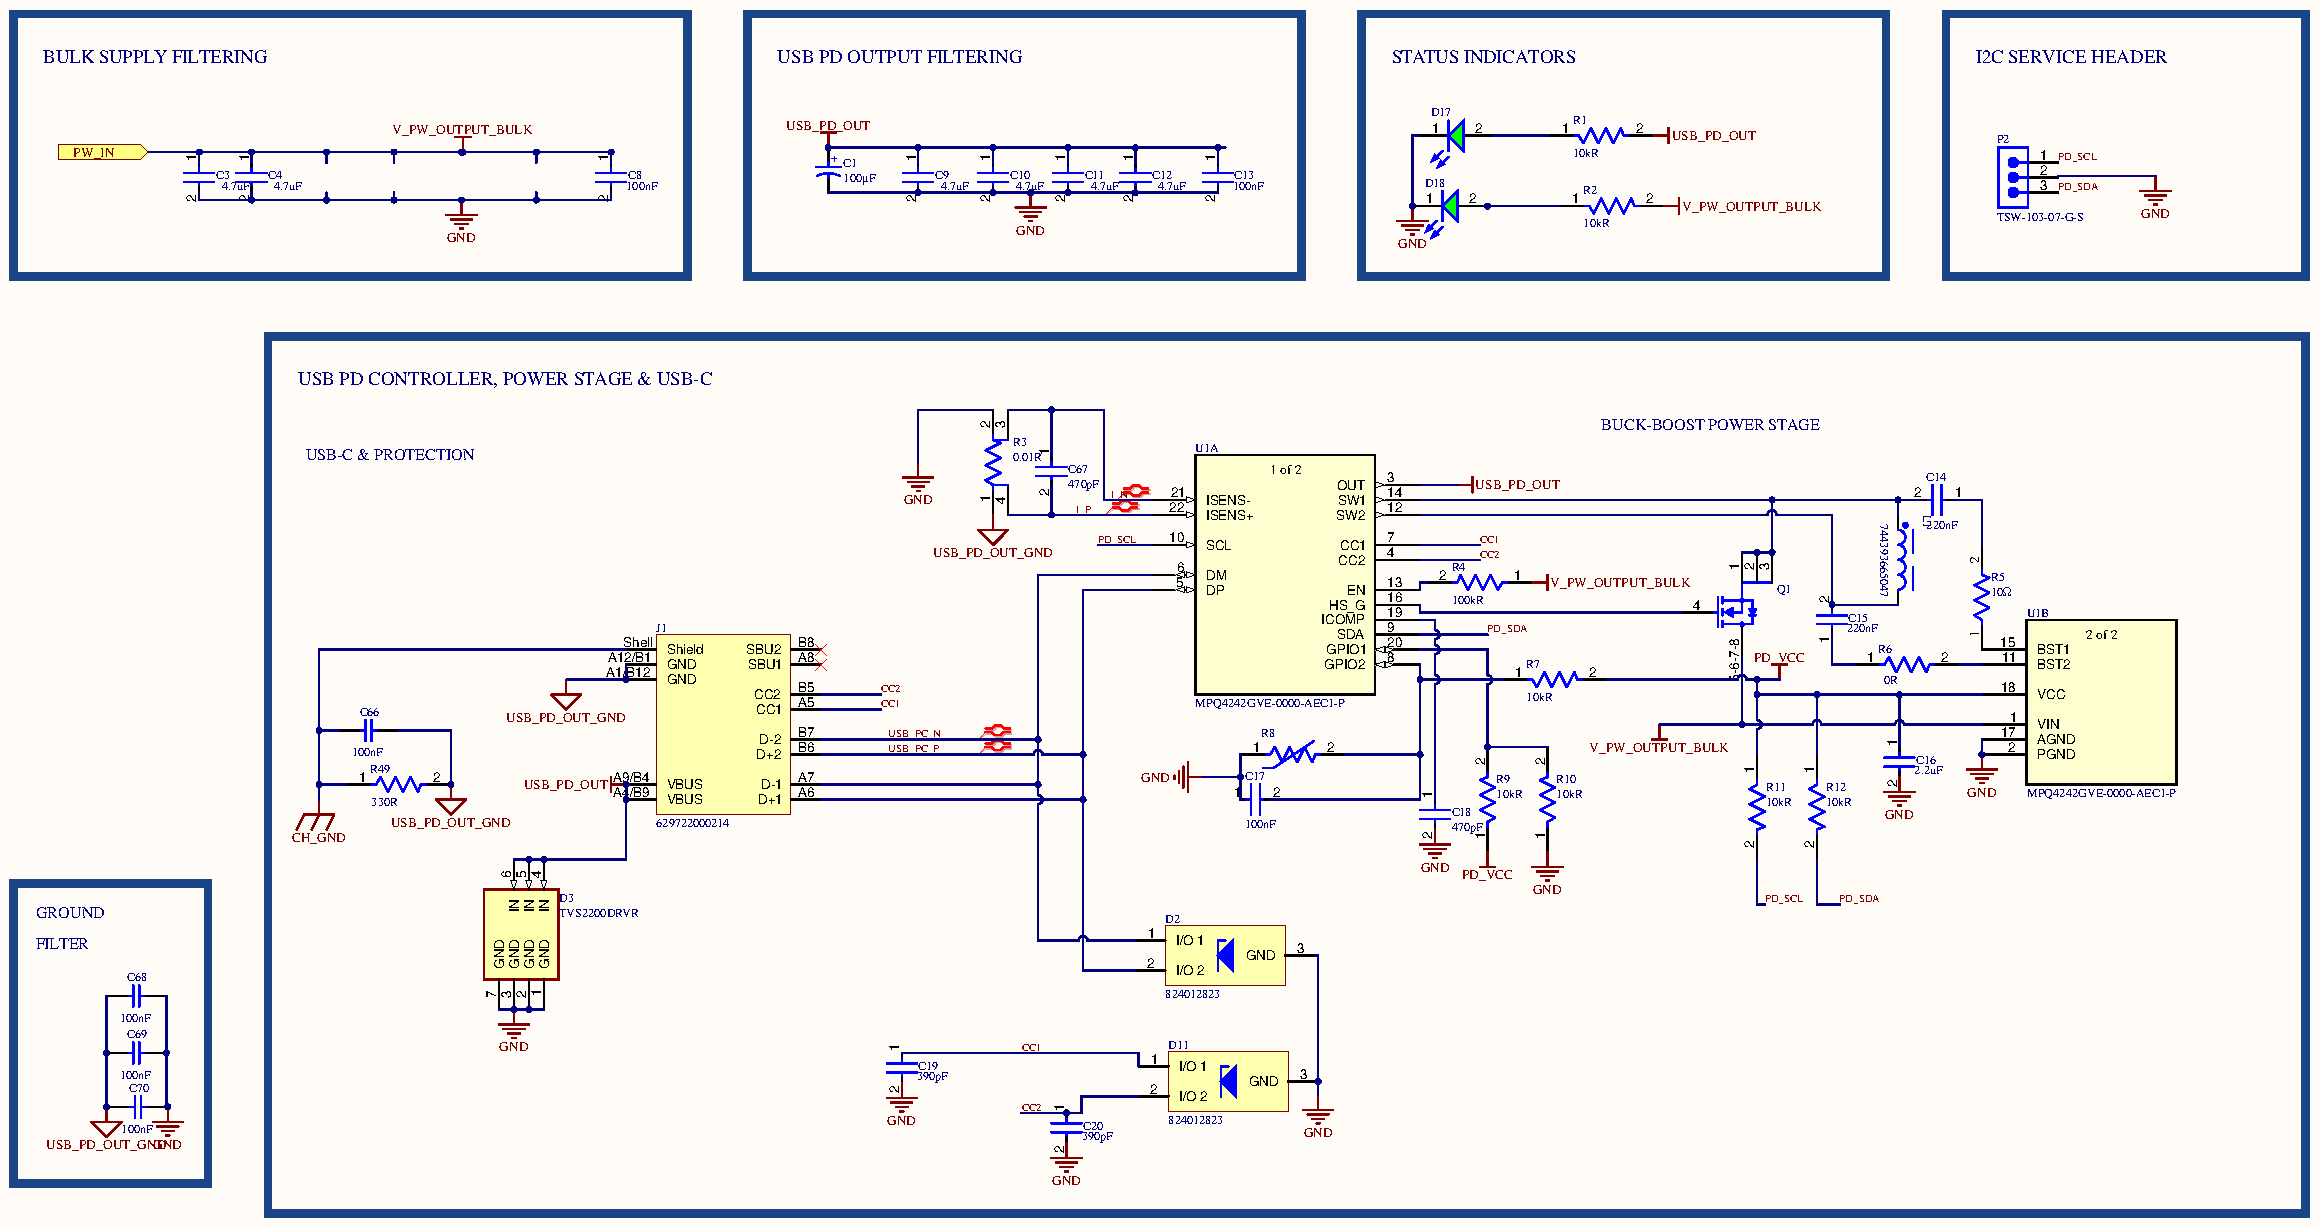
\includegraphics[width=0.97\linewidth,height=0.76\textheight,keepaspectratio]{Pictures/Thesis/07_Hardware/Rebuilt/schematic_v2_usb_excerpt.pdf}
\caption{V2 sheet 2: MPQ4242 output stage, USB-C connector, current sensing, capacitors, and interface protection.}
\label{fig:schematic-usbc}
\end{figure}
\end{landscape}

The \SI{5}{\volt}, \SI{9}{\volt}, \SI{15}{\volt}, and \SI{20}{\volt} fixed outputs were tested. According to the project notes, the \SI{20}{\volt} setting is advertised for up to \SI{5}{\ampere}. A \SI{100}{\watt} operating point was not reached in the completed tests.

The MCU regulates the secondary bulk voltage using feedback at PA1. The USB-C PD stage regulates its output to the selected PD level. Voltage at the load can differ because of cable drop, so the measurement point is stated with each result. The fixed-output tests confirmed operation of the assembled path at those settings. USB-PD negotiation and interoperability still need protocol testing.

\section{Analog Feedback and MCU Inputs}
\label{sec:hw-sensing}

On the V1.0 test platform, the controller acquires scaled primary voltage at PA0, isolated secondary-bulk voltage at PA1, and the LMG2652 half-bridge-current signal at PA2. TLV9064 buffers reduce ADC loading of the sensing circuits. The AMC0330 transfers secondary-voltage feedback across the isolation barrier to the primary-side MCU. V2 uses the same measurements with direct ADC connections, as shown in \Cref{fig:schematic-mcu}.

\begin{figure}[htbp]
\centering
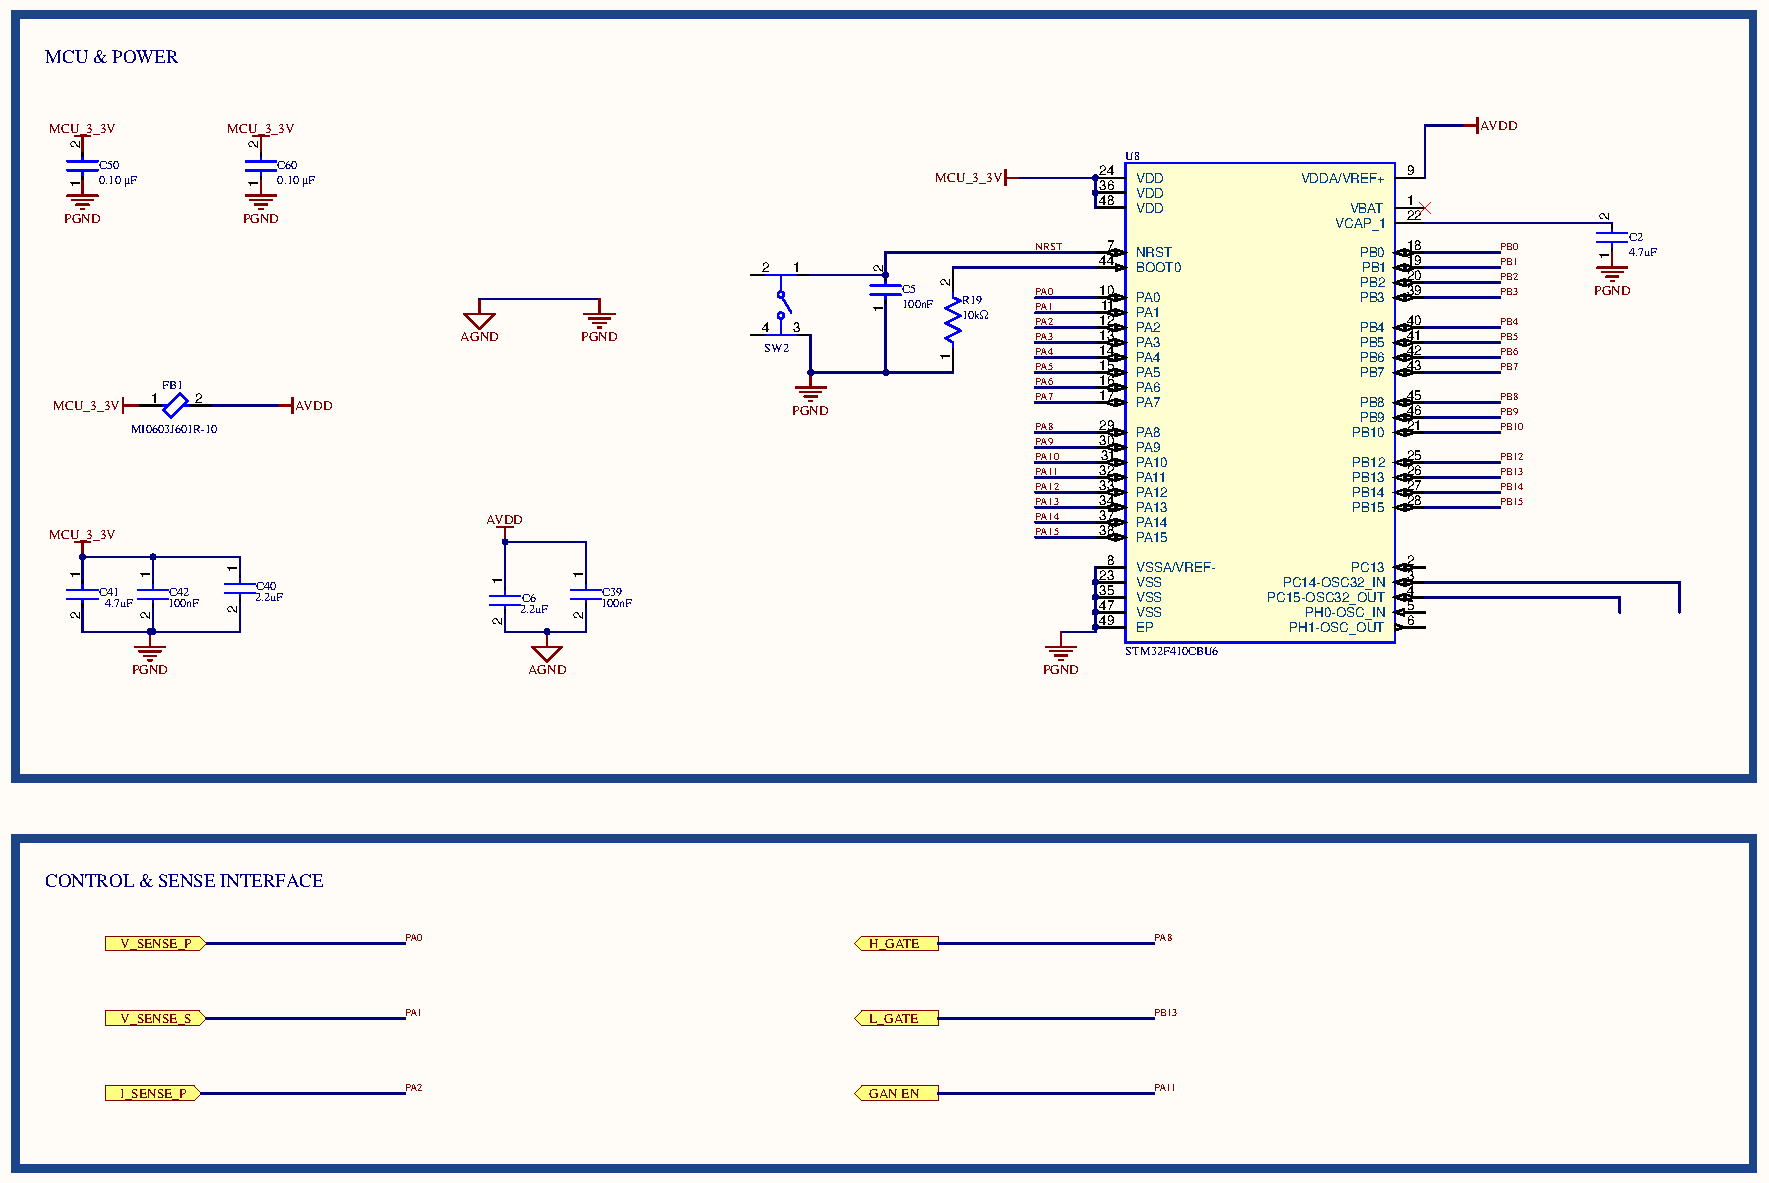
\includegraphics[width=\textwidth,height=0.57\textheight,keepaspectratio]{Pictures/Thesis/07_Hardware/Rebuilt/schematic_v2_controller_excerpt.pdf}
\caption{V2 sheet 4 MCU connections. Feedback enters pins PA0--PA2 directly; PA8/PB13 provide carrier commands and PA11 provides burst enable. The MCU uses the primary-side ground reference.}
\label{fig:schematic-mcu}
\end{figure}

\begin{table}[htbp]
\centering
\caption{MCU feedback pins and their functions.}
\label{tab:hw-sensing-evidence}
\begin{tabularx}{\textwidth}{@{}p{0.12\textwidth}p{0.32\textwidth}X@{}}
\toprule
MCU pin & Input & Firmware function\\
\midrule
PA0 & Primary-voltage feedback & Diagnostics and optional high-line duty reduction\\
PA1 & Isolated secondary-bulk voltage & Voltage regulation and overvoltage protection\\
PA2 & Half-bridge current sensing & Load detection, diagnostics, and optional current protection\\
\bottomrule
\end{tabularx}
\end{table}

The half-bridge-current signal at PA2 was used for load classification. Its product with secondary voltage at PA1 does not represent connector output power without a validated conversion model. Output power was therefore calculated from external VBUS and load-current measurements, while the controller regulated secondary-bulk voltage.

V1.0 includes an external \SI{2.5}{\volt} reference, omitted in V1.1, while the final firmware defaults to a \SI{3.3}{\volt} ADC reference. Divider ratios, amplifier scale, buffers, gain, and offset also affect the conversion, so the scales must be checked against measured circuit and ADC-pin voltages. The calibration settings are given in \Cref{sec:ctrl-feedback}.

\section{Protection Layers}
\label{sec:hw-protection}

The hardware and firmware handle different faults. The input fuse and varistor act at the AC connection. The discharge circuit and output TVS devices address stored voltage and output transients. The LMG2652 includes undervoltage, cycle-by-cycle overcurrent, and overtemperature functions \cite{tiLMG2652}. Startup control, bounded burst-enable commands on the original prototype's MCU output PA10, no-load energy limits, and latched overvoltage or optional current faults were added in firmware.

Device protection and firmware thresholds act on different quantities; neither the internal current limit nor the PA2 signal measures connector output current. The PA2 firmware trip is disabled by default, and the active voltage loop does not call the legacy current-foldback helper. Soft and hard overvoltage decisions are described in \Cref{sec:ctrl-faults}.

These layers were used during supervised laboratory testing. The response from fault detection through shutdown and recovery still needs to be measured. Product qualification would also require checks of redundancy and single-fault response.

\section{Auxiliary Supplies and Startup}
\label{sec:hw-aux}

Startup depends on the auxiliary supplies. The primary bias rail is supplied by BAC1S12SC, and the local controller and sensing circuits are powered by LMR54410 regulators. The isolated feedback and output electronics use secondary power. The MCU can therefore start before the isolated sensing circuit is powered sufficiently to provide a valid reading.

The local supply rails, UART communication, inhibited burst-enable output PA10, carrier outputs, and analog feedback were checked during bring-up before the loop was closed. The LMG2652 bias must be within its operating range before switching.

Bounded precharge bursts and settling intervals are used to power the secondary-side sensing before normal control. The sequence ends at the readiness threshold or attempt limit (\cref{sec:ctrl-state}). Auxiliary-rail startup, operating range, and temperature rise require further measurement.

\section{PCB Layout and Current Paths}
\label{sec:hw-layout}

The four-layer V1.0 board was arranged to follow the power path. The AC input is on the left, followed by the central charge pump and GaN stage, then the magnetics, rectifier, output, and control sections. The manufactured layout is shown in \Cref{fig:pcb-v1-0-placement-reference,fig:pcb-v1-0-layout-overview}.

\begin{figure}[htbp]
\centering
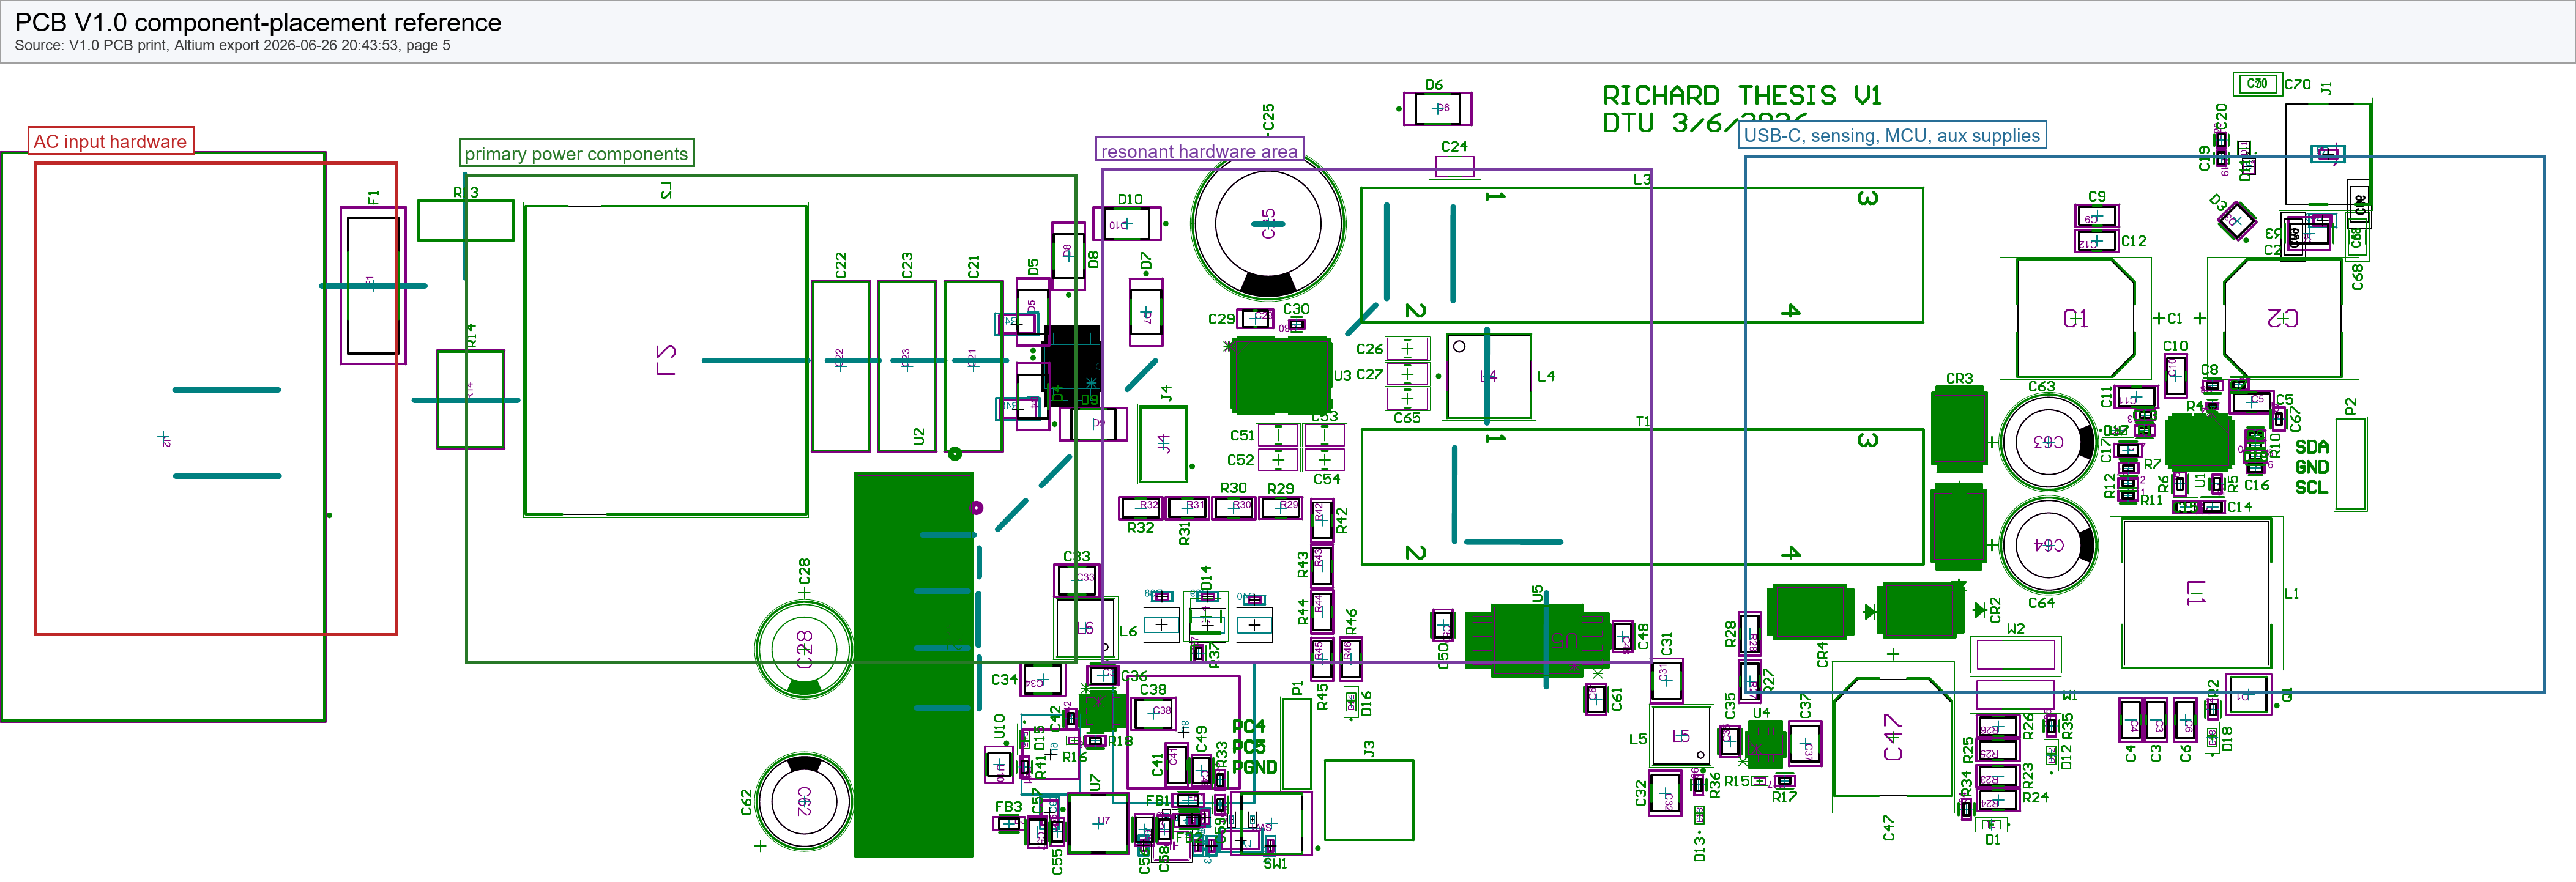
\includegraphics[width=\textwidth]{Pictures/Thesis/07_Hardware/pcb_v1_0_component_placement_reference.png}
\caption{V1.0 component placement. The AC input, high-frequency power stage, magnetics, and output/control circuits are marked.}
\label{fig:pcb-v1-0-placement-reference}
\end{figure}

\begin{figure}[htbp]
\centering
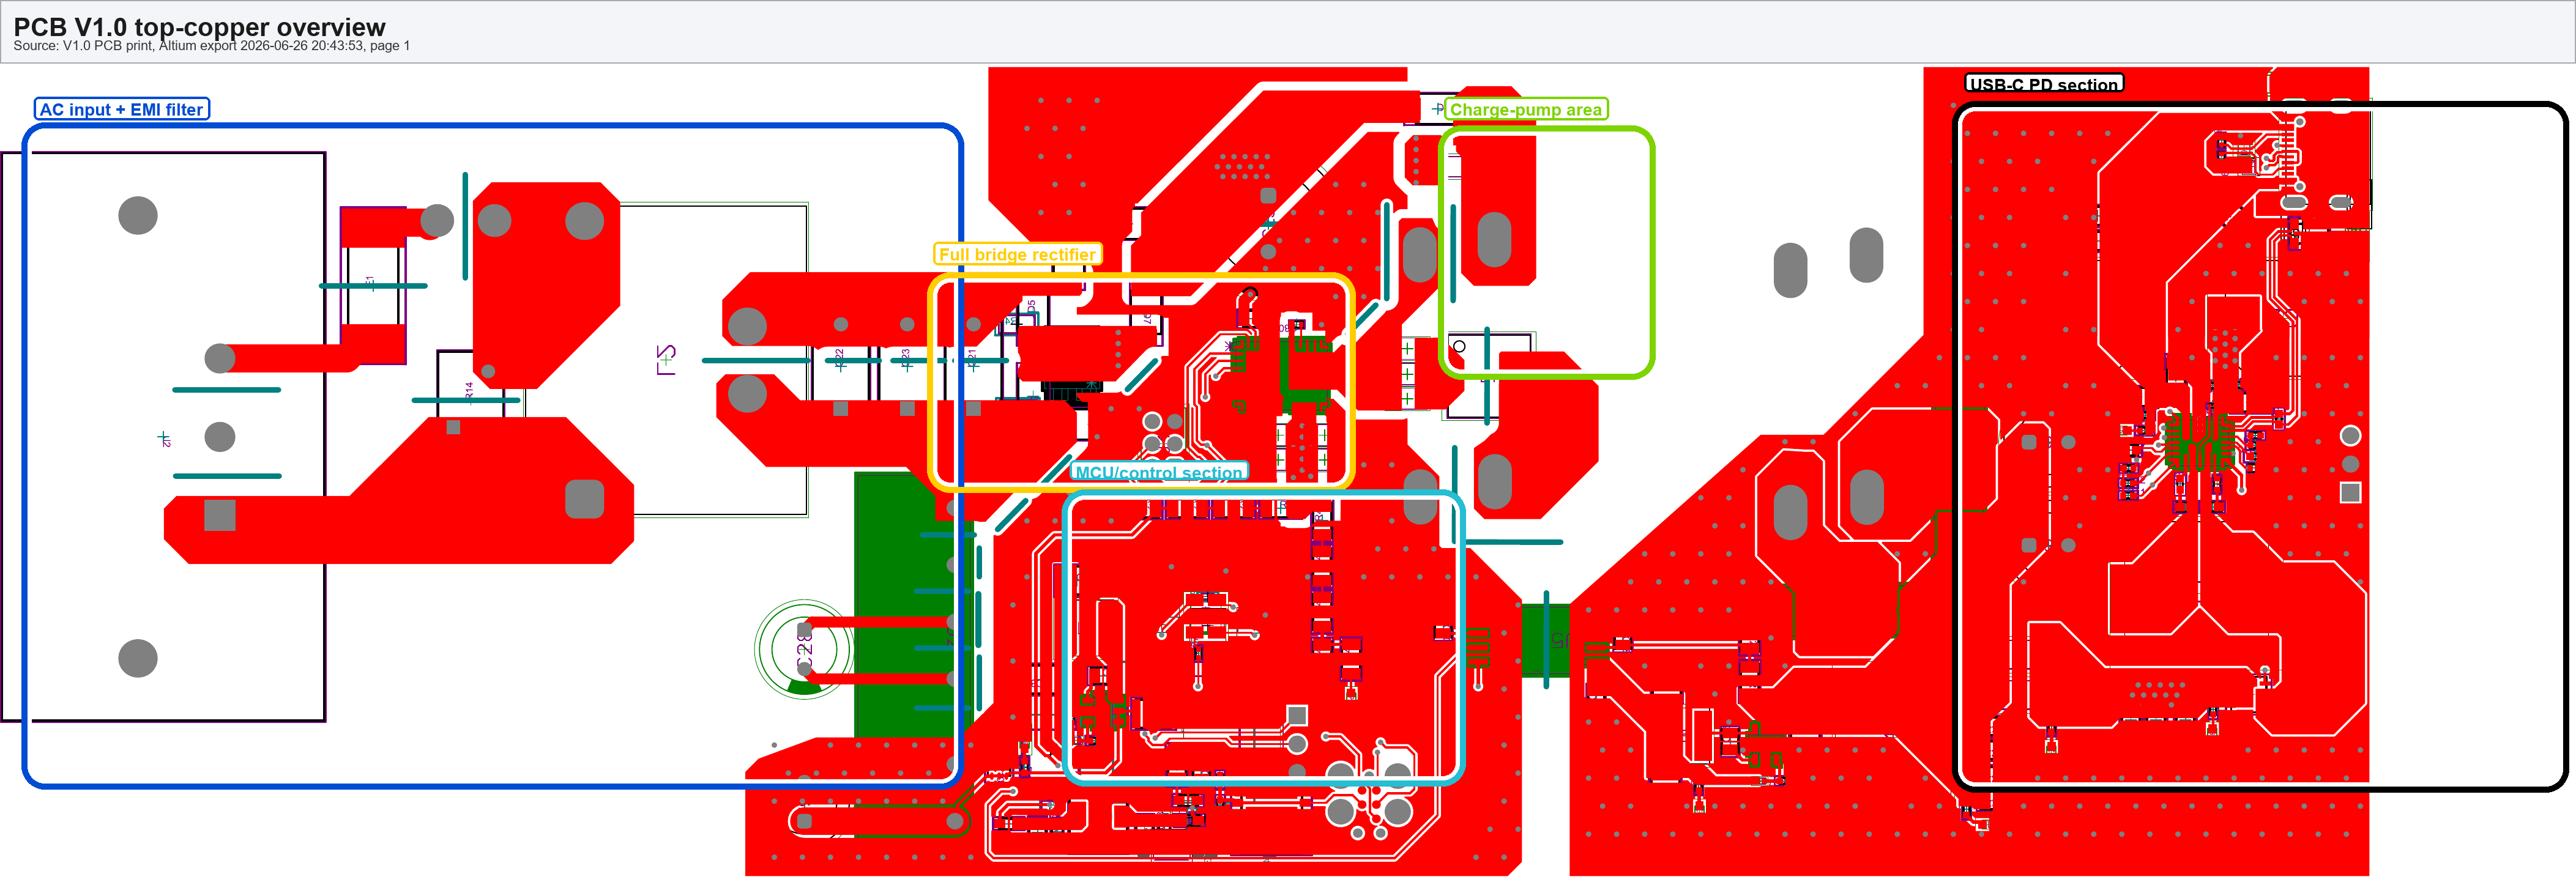
\includegraphics[width=\textwidth]{Pictures/Thesis/07_Hardware/pcb_v1_0_top_copper_overview_annotated_v2.png}
\par\smallskip
\small (a) Top copper and principal component regions.
\par\medskip
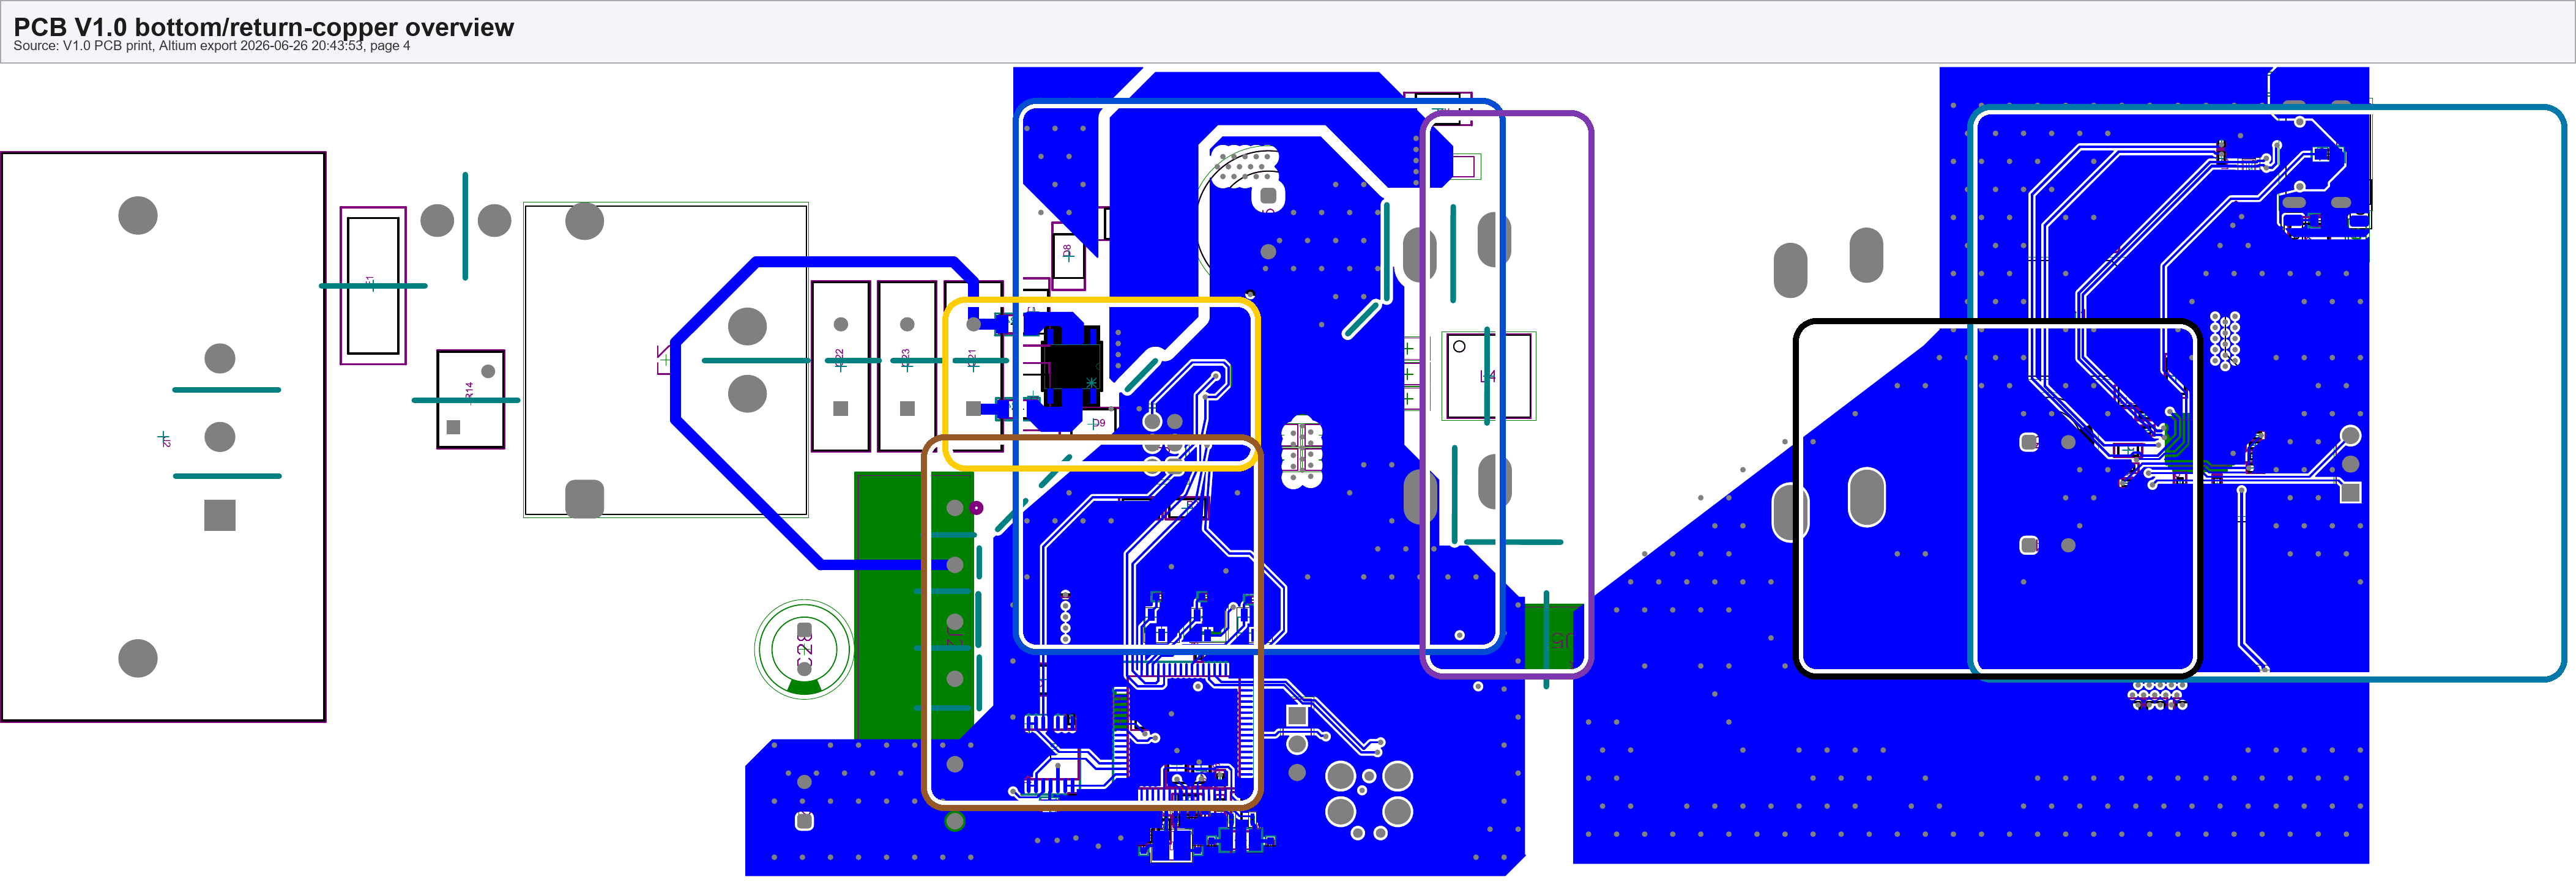
\includegraphics[width=\textwidth]{Pictures/Thesis/07_Hardware/pcb_v1_0_bottom_return_overview_annotated_v2.png}
\par\smallskip
\small (b) Bottom copper and return paths.
\caption{V1.0 top and bottom copper, showing component regions and return paths.}
\label{fig:pcb-v1-0-layout-overview}
\end{figure}

At \SI{1}{\mega\hertz}, parasitic inductance depends on the complete loop. The half-bridge loop closes through its local link decoupling and return. The resonant loop closes through the transformer connections, while the pump capacitor and diodes carry link-charging pulses. Added inductance can change both overshoot and the current available during dead time.

The high-\(dv/dt\) node also couples into nearby copper. Its position relative to the sensing and transformer connections affects analog noise and common-mode current. The return paths must therefore be considered along with the signal traces. These paths are shown in the annotated views. Loop inductance and common-mode capacitance still need to be measured to quantify their contribution.

The final series-inductor connections differ from the original footprint. Their length and support affect the tested tank impedance and must be reproduced along with the component values. The carrier-pin correction showed another layout dependency: the MCU pin on the drawing must support the required timer output.

Clearance of \SI{1}{\milli\metre} and creepage of \SI{3}{\milli\metre} were specified for the relevant nets. The insulation was then checked in the laboratory. A full assessment must also cover the installed transformer, working voltage, material assumptions, and standardized dielectric testing.

\subsection{Electromagnetic Coupling}
\label{sec:hw-emi}

The high-frequency stage has several coupling paths. VSW transitions, pump current, tank current, and secondary rectifier commutation generate noise, while the MCU enable output PA10 on the original prototype adds the slower burst envelope. The burst pattern and control state change the resulting frequency content.

The resulting noise current can return through the input filter, pass through transformer capacitance, or couple into the output cable and bench wiring. Cable placement, grounding, source impedance, load, and duty must therefore be defined for an emissions test. Conducted or radiated emissions were not measured with a line-impedance stabilization network and calibrated receiver. That test is needed to measure the margin to an emissions limit.

\subsection{Thermal Paths}
\label{sec:hw-thermal}

The assembly was tested without an enclosure. Heat was spread through the PCB copper and removed by ambient convection. The heat sources include the GaN stage, resonant inductors, planar magnetics, rectifier, MPQ4242 stage, and auxiliary regulators. An enclosure or dedicated heat sink would change these paths, so continuous output would need to be retested.

Heat leaves the GaN device through its bottom pad and board copper. The resonant and secondary components also dissipate heat; the two series inductors share the branch loss while carrying the same current. Thermal images at the labeled loads and measured surfaces are discussed in \Cref{sec:res-thermal}, using the method in \cref{sec:method-thermal}. Test duration and ambient conditions were not fully recorded for the high-power captures, so component temperatures still need to be recorded over time to check sustained operation.

\section{Components and Bring-Up Changes}
\label{sec:hw-bom}

The fitted components are listed in \Cref{tab:hw-bom-provenance}. The board photographs show the resonant-branch changes made during bring-up.

\begin{table}[H]
\centering
\caption{Main components fitted to the prototype.}
\label{tab:hw-bom-provenance}
\small
\begin{tabularx}{\textwidth}{@{}p{0.25\textwidth}p{0.34\textwidth}X@{}}
\toprule
Function & Part & Value or function\\
\midrule
Input fuse & 04653.15DR & \SI{3.15}{\ampere}, \SI{250}{\volt} AC\\
Varistor & ERZV07D471 & Surge clamping\\
Input choke & 7448680200 & Two \SI{120}{\micro\henry} windings on V1.0\\
Pump capacitor & C1206X202FBGACTU & \SI{2}{\nano\farad}, \SI{630}{\volt}\\
DC-link capacitor & 860241478004 & \SI{22}{\micro\farad}, \SI{450}{\volt} fitted to the prototype\\
Pump diodes & PU1JLWH & Ultrafast steering rectifiers\\
GaN stage & LMG2652RFBR & Integrated half bridge and drivers\\
Final resonant branch & Two 7443640470B & \SI{9.4}{\micro\henry} nominal series total\\
Controller & STM32G071RBT6 & Carrier, enable timing, ADC DMA, and UART\\
Isolated voltage sensing & AMC0330 & Secondary-bulk feedback\\
Output stage & MPQ4242GVE-0000-AEC1-P & USB-C PD voltage regulation and interface\\
\bottomrule
\end{tabularx}
\end{table}

\begin{figure}[htbp]
\centering
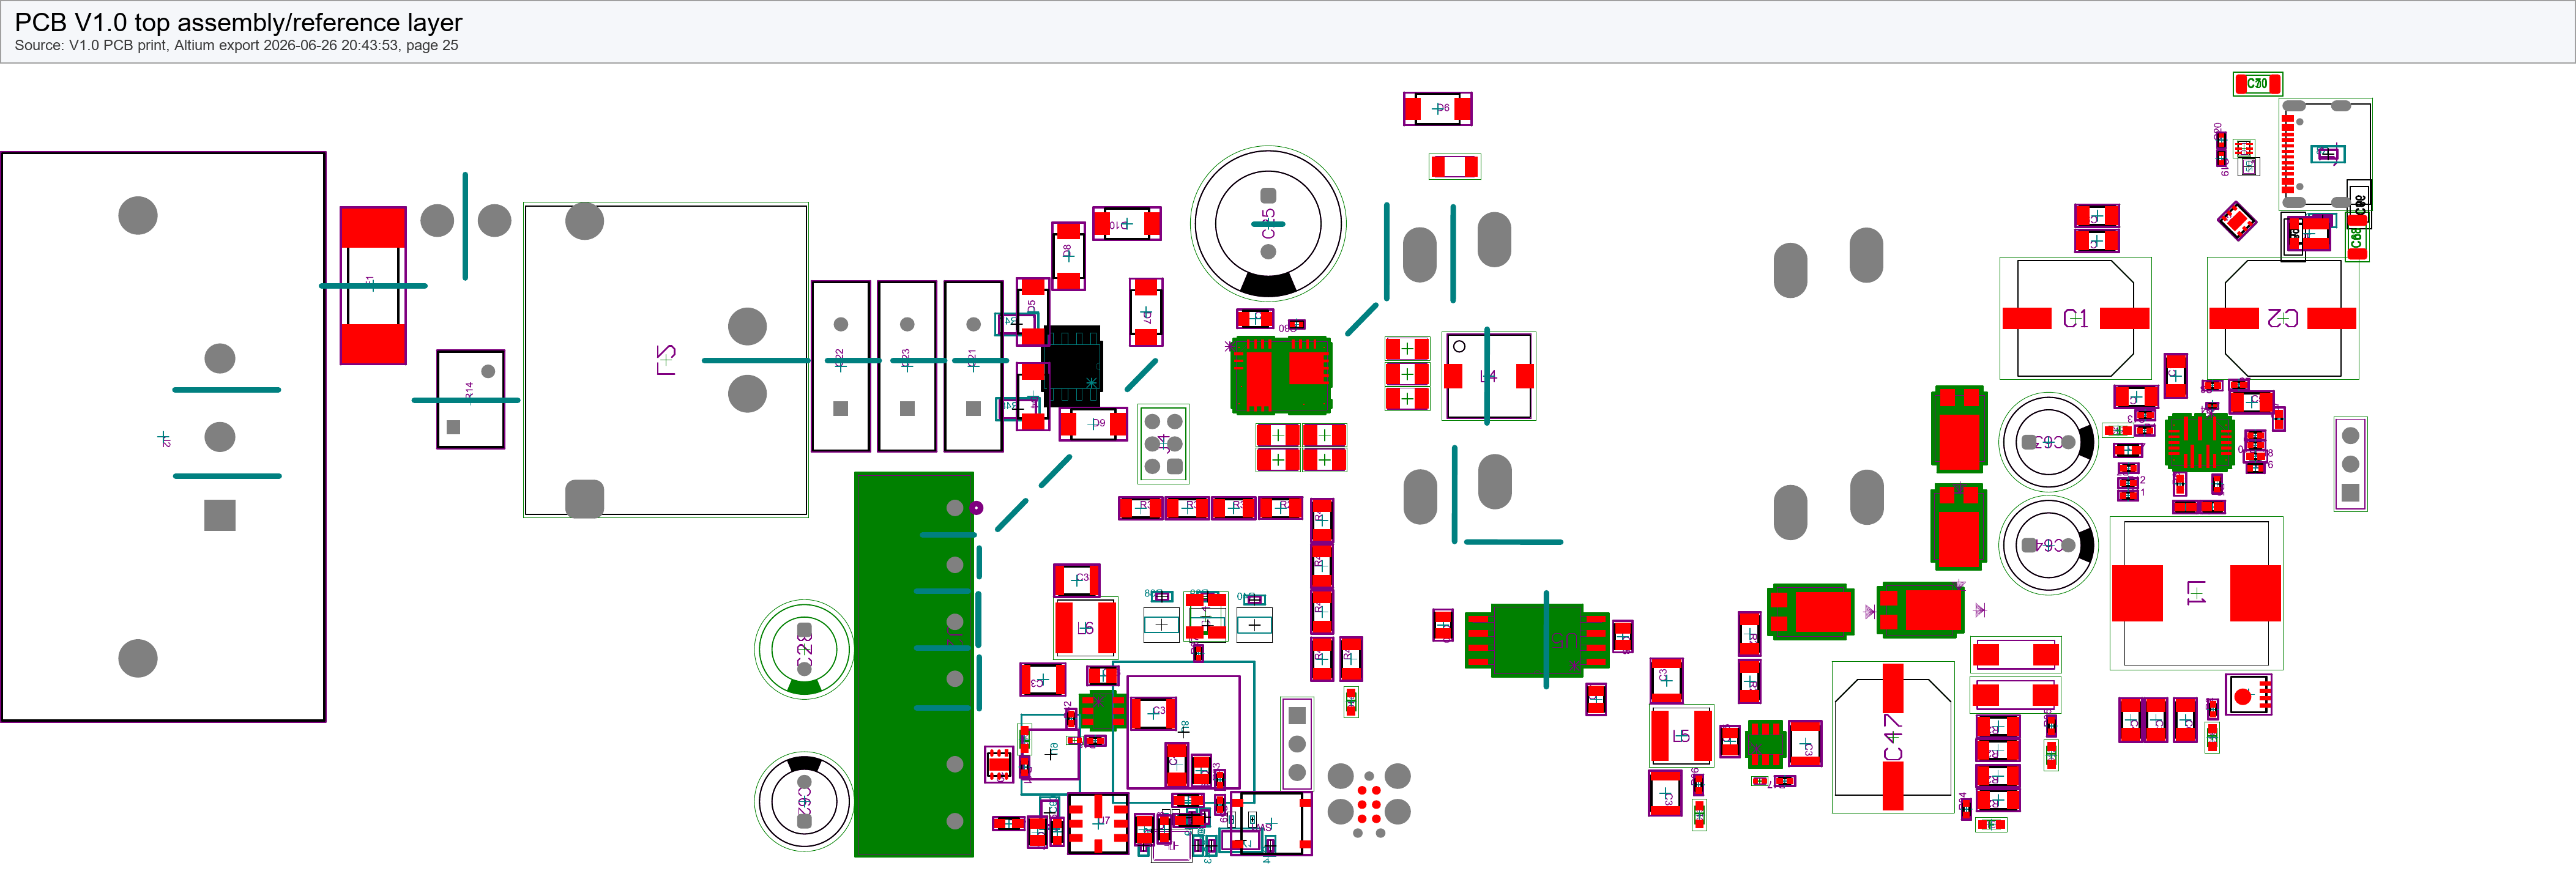
\includegraphics[width=\textwidth]{Pictures/Thesis/07_Hardware/pcb_v1_0_top_assembly_reference.png}
\caption{V1.0 top-side assembly drawing.}
\label{fig:pcb-v1-0-top-assembly-reference}
\end{figure}

\begin{table}[H]
\centering
\caption{Circuit and feedback corrections made during bring-up.}
\label{tab:hardware-implementation-lessons}
\begin{tabularx}{\textwidth}{@{}p{0.23\textwidth}X@{}}
\toprule
Item & Correction\\
\midrule
Carrier pins & PA8/PA9 form the final fixed carrier pair; PA10 provides enable. The corrected pins are shown in V1.1.\\
Charge-pump drawing & V1.1 shows the corrected diode connection and component substitutions.\\
Resonant branch & Final tests use two \SI{4.7}{\micro\henry} inductors in series.\\
PA2 feedback & The half-bridge-current signal is used for load detection; it is not the USB-C output current.\\
\bottomrule
\end{tabularx}
\end{table}

The final measurements apply to the modified V1.0 assembly and series-inductor arrangement shown here. The fitted components, calibration, and runtime settings must be reproduced along with the PCB revision.

\subsection{V1.1 Circuit Corrections and V1.2 Layout}
\label{sec:hw-unmanufactured-revisions}

The circuit corrections were included in V1.1, followed by a more compact V1.2 layout. That layout was not manufactured or tested during this project.

\begin{table}[H]
\centering
\caption{Later circuit and layout revisions.}
\label{tab:unmanufactured-board-revisions}
\begin{tabularx}{\textwidth}{@{}p{0.16\textwidth}X@{}}
\toprule
Revision & Status and use\\
\midrule
V1.1 & Drawing corrections and component changes; no separate test board was built\\
V1.2 & More compact layout; not built or tested\\
\bottomrule
\end{tabularx}
\end{table}

The later drawings show the circuit changes and intended next layout. The power, temperature, regulation, and power-quality measurements apply to the manufactured V1.0 assembly. Each new board must be brought up and measured separately to check whether the earlier results still apply.

\section{V2 Hardware and MCU Integration}
\label{sec:hw-v2}

V2 integrates the MCU, power stage, sensing, local supplies, and USB-C output on a four-layer PCB \cite{ststm32f410ds}.

The nominal \SI{1}{\mega\hertz} carrier and burst-enable control were retained from the earlier DMA-based controller (\cref{ch:control}). Board-dependent peripherals were ported before browser telemetry and commands were added. The later V2 firmware adds output-OFF adjustment of carrier frequency and dead time (\cref{sec:ctrl-v2-adjustable-timing}).

\subsection{V2 PCB and Physical Integration}

The V2 PCB was designed with four copper layers: Top Layer, Int1
(GND), Int2 (PWR), and Bottom Layer. Components are placed on both sides.
The input and high-voltage power circuitry occupy one end of the board,
the planar-magnetic connections occupy the central region, and the USB-C
output is at the opposite end. The planar-magnetic boards are mounted
upright in the mechanical design. The controller, sensing, local supplies,
and external resonant inductor are also distributed across the two sides.
Figure~\ref{fig:v2-pcb-layout-overview} shows the top and bottom copper prints.
The complete layer, assembly, mask, and drill prints are included with the
schematic in Section~\ref{sec:app-v2-oct27}.

\begin{figure}[p]
\centering
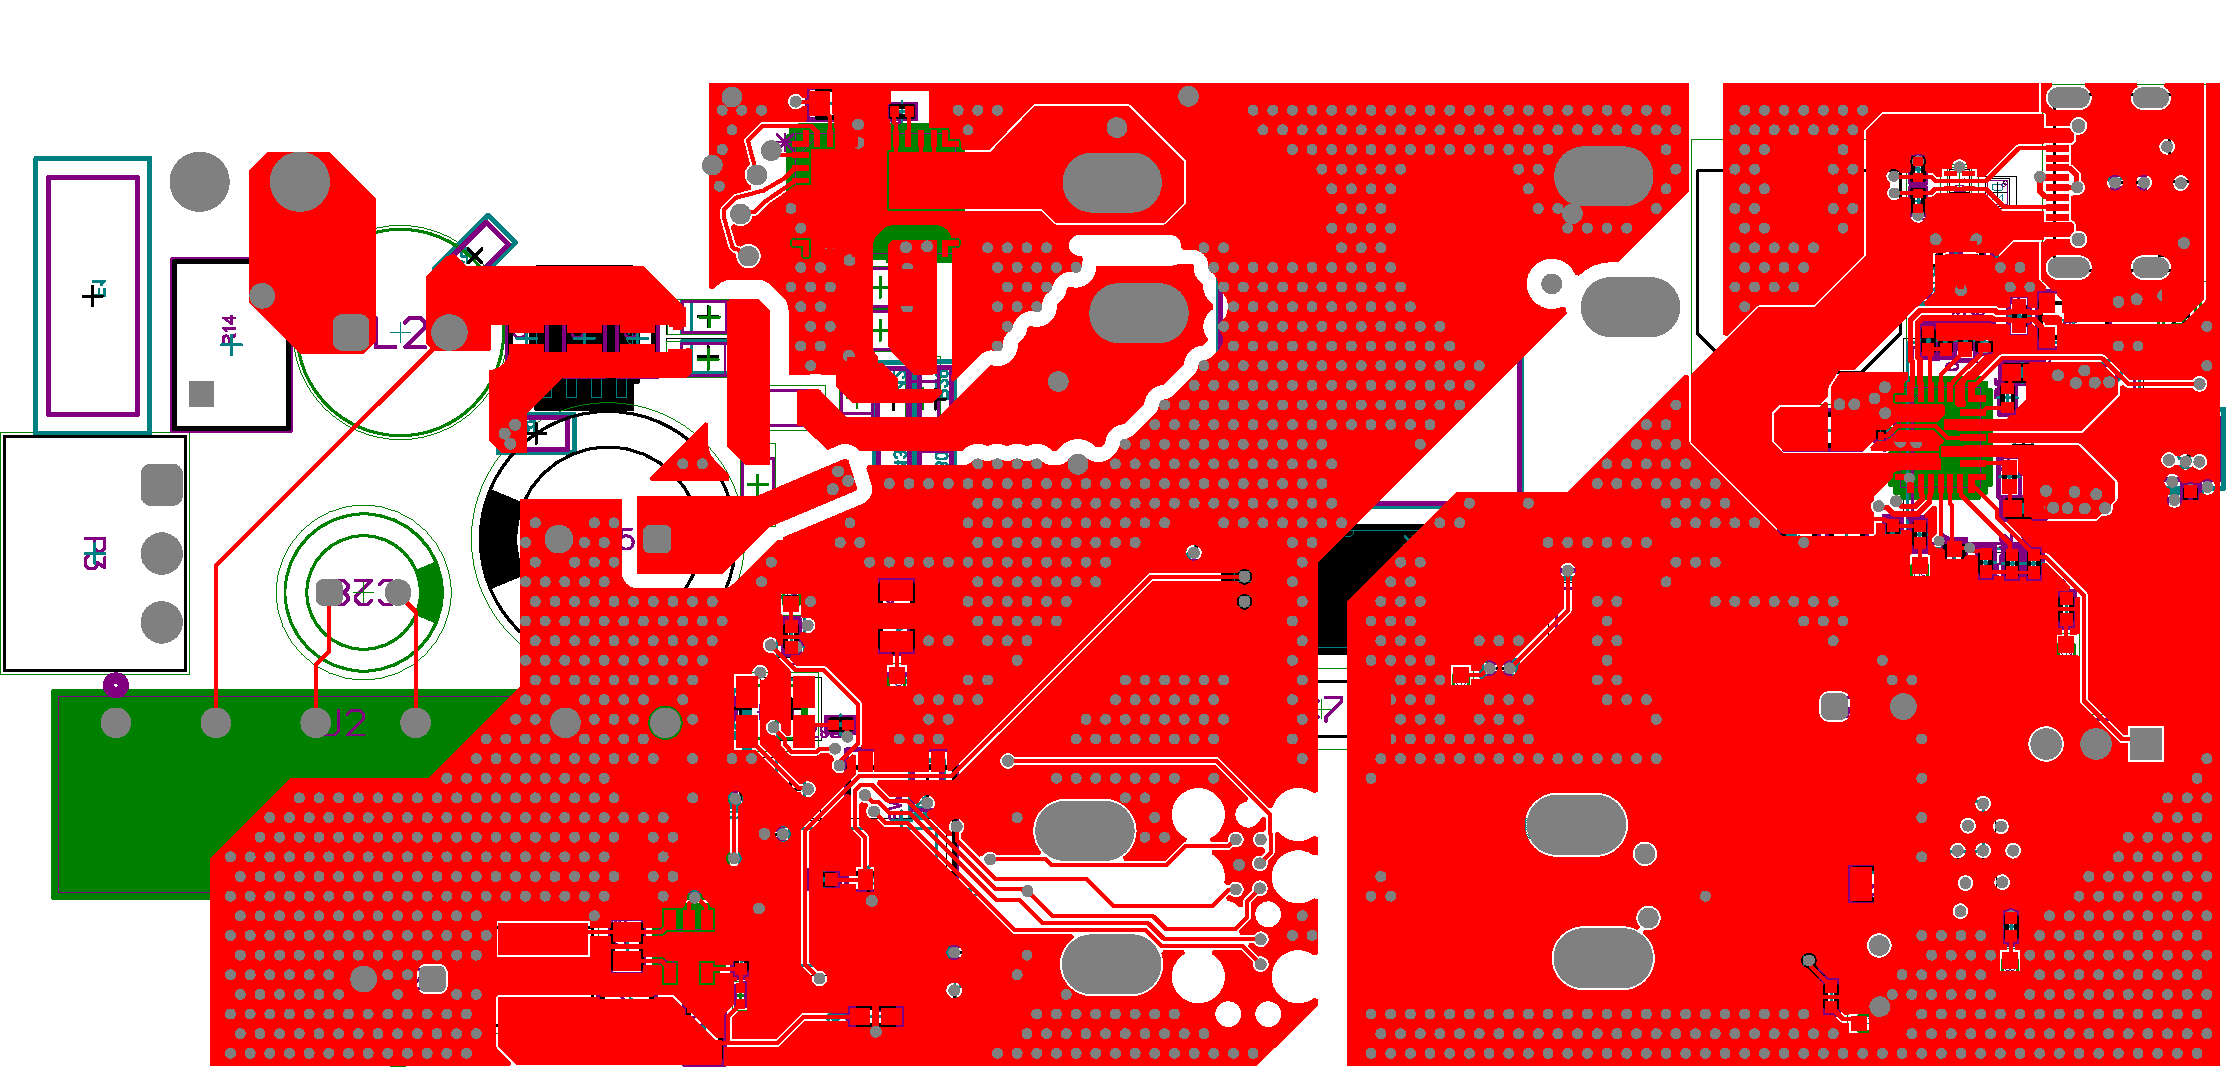
\includegraphics[page=1,width=\linewidth,height=0.33\textheight,keepaspectratio]{Pictures/Thesis/07_Hardware/PCB_V2_F410_2026-10-27.pdf}

\vspace{0.8em}
\includegraphics[page=4,width=\linewidth,height=0.33\textheight,keepaspectratio]{Pictures/Thesis/07_Hardware/PCB_V2_F410_2026-10-27.pdf}
\caption{V2 top copper (upper) and bottom copper (lower), shown in the same orientation.}
\label{fig:v2-pcb-layout-overview}
\end{figure}
\FloatBarrier

The finished board dimensions, assembly height, copper weights, and layer
thicknesses are not specified in the PCB drawings. V2 power density
therefore requires separate assembly measurements. The L4 footprint belongs
to the original resonant branch. The external inductor was removed during
the later leakage-only test described in \cref{sec:res-v2-testing}.

\subsection{Controller Connections and Timing}

The V2 carrier uses TIM1 CH1/CH1N at PA8/PB13. Moving the low-side command from PA9 and burst enable from PA10 to PA11 releases PA9/PA10 for USART1 TX/RX. Thus PA10 serves as burst enable on the G071 platform and serial receive on the F410. \Cref{tab:hw-v2-pinmap} lists the MCU pins from sheet 4 and their package pin numbers.

\begin{table}[H]
\centering
\caption{MCU pins on the G071 controller and V2 F410. Package pin numbers in the V2 column apply to the F410CBU6.}
\label{tab:hw-v2-pinmap}
\small
\begin{tabularx}{\textwidth}{@{}p{0.24\textwidth}p{0.21\textwidth}X@{}}
\toprule
Function & G071 pins & V2 F410 pins\\
\midrule
High-side carrier & PA8 & PA8, pin 29; TIM1 CH1\\
Low-side carrier & PA9 & PB13, pin 26; TIM1 CH1N\\
Power-stage enable & PA10 & PA11, pin 32; TIM5 schedules GPIO edges\\
Command UART & PC4 TX / PC5 RX & PA9 TX / PA10 RX, pins 30 / 31; J3 pins 5 / 6\\
Primary voltage & PA0 & PA0, pin 10; ADC1 channel 0\\
Secondary-bulk voltage & PA1 & PA1, pin 11; ADC1 channel 1\\
Half-bridge-current signal & PA2 & PA2, pin 12; ADC1 channel 2\\
\bottomrule
\end{tabularx}
\end{table}

The earlier V2 port configures center-aligned TIM1 at a nominal \SI{100}{\mega\hertz} timer clock, with auto-reload ARR = 50, compare CCR1 = 25, and dead-time field DTG = 4. These settings give a nominal \SI{1}{\mega\hertz} complementary carrier and \SI{40}{\nano\second} programmed dead time \cite{ststm32f410rm}. TIM5 schedules the enable envelope; bounded polling of carrier updates attempts to align non-static transitions but leaves software-dependent edge latency. The later powered trial used a reported \SI{60}{\nano\second} software setting (\cref{sec:res-v2-testing}), with its firmware version unrecorded. Effective dead time and enable alignment are measured from driver-input and switch-node captures.

ADC1 continuously scans primary voltage at PA0, secondary-bulk voltage at PA1, and half-bridge current at PA2 through DMA2 Stream0 Channel0 without synchronization to the carrier. At the \SI{25}{\mega\hertz} ADC clock, 84 acquisition and 12 conversion cycles give calculated intervals of \SI{3.84}{\micro\second} per channel and \SI{11.52}{\micro\second} per frame. Secondary-bulk voltage remains the regulated quantity; primary current supports load classification and optional protection rather than connector output-current measurement.

\subsection{Power Circuit, Sensing, and Local Supplies}

Power sheet 3 includes the LMG2652RFBR GaN half bridge, AMC0330 isolated feedback, BAC1S12SC bias supply, and two LMR54410DBVR regulators. D4, D5, D9, and D10 form the input bridge; D6--D8 form the pump diode network. All seven are labeled S4D02120T in the drawing. C25 is connected across the pumped HVVCC link, downstream of the input bridge. The primary regulator supplies \texttt{MCU\_3\_3V}; the secondary supplies \texttt{SEC\_3\_3V}. C29 is specified as \SI{1}{\micro\farad} at AUX and C30 as \SI{22}{\nano\farad} at bootstrap. The drawing also includes CAP300DG discharge, the \SI{100}{\micro\henry} L2 input inductor, three \SI{10}{\nano\farad} capacitors C21--C23, the \SI{2}{\nano\farad} C24 pump capacitor, and the \SI{10}{\micro\farad} C25 link capacitor. The parts fitted to the assembled V2 still need to be checked against the drawing.

In the resonant branch, L4 is labeled SER1512-103MED, with a nominal value of \SI{10}{\micro\henry}, but complete values or part definitions are missing for L3, T1, and C26. The external series inductor used in preliminary powered tests was reported at approximately \SI{9.4}{\micro\henry} (\cref{sec:res-v2-testing}); whether it was the component fitted at L4 has not been confirmed. The final V1.0 arrangement used two \SI{4.7}{\micro\henry} series inductors. The fitted V2 branch and transformer must be checked before calculating resonance or comparing switching waveforms.

MCU sheet 4 omits the TLV9064 buffers and connects the feedback nets directly to PA0--PA2. ADC loading and settling must therefore be checked with the actual source impedance. The code assumes a \SI{1.50}{\mega\ohm}/\SI{10}{\kilo\ohm} primary ladder, a \SI{390}{\kilo\ohm}/\SI{10}{\kilo\ohm} secondary divider, and \SI{3.3}{\volt} ADC/AMC references. R50 is labeled \SI{820}{\ohm} between the LMG2652 current-sense node and primary ground.

The divider labels do not agree with those assumptions. R29--R32 are each labeled \SI{6.2}{\mega\ohm}, and R27--R28 have the same value. Taken literally, the primary and secondary ratios are 4:1 and 2:1. These ratios do not support the intended \SI{450}{\volt} primary and \SI{28}{\volt} secondary ranges. The fitted resistor values and gain from each measured node to its ADC pin still need to be checked. Displayed voltages and voltage-protection thresholds are reliable only when the firmware conversion scales match the measured circuit.

USB-PD sheet 2 includes the MPQ4242GVE-0000-AEC1-P output stage, fed from \texttt{V\_PW\_OUTPUT\_BULK} and supplying \texttt{USB\_PD\_OUT}. The \SI{0.01}{\ohm} connector current-sense resistor is R3. This is separate from the LMG2652 sensing path on PA2. Further power-path and USB-PD tests are still needed after the preliminary powered tests in \cref{sec:res-v2-testing}.

\Needspace{0.30\textheight}
\subsection{V2 Checks and Remaining Measurements}

The October plan reports a V2 operating point near \SI{85}{\watt} and a \SI{100}{\watt} target \cite{projectOctoberPlan}. The assembly, input power, output voltage/current, temperature, duration, and firmware settings were not recorded together, so the point must be repeated with these conditions recorded. It is not included in the measured curves.

The matched \SI{79.89}{\watt} tests on the modified V1.0 assembly provide a connector-output baseline (\cref{ch:results}). Later V2 secondary-output tests reached higher power with voltage droop and continued heating (\cref{sec:res-v2-testing}); thermal-endurance tests remain incomplete. The V1.0 outline is \SI{202.77}{\milli\metre} by \SI{72.77}{\milli\metre}; V2 assembly dimensions must be measured separately before calculating its power density.

\section{V3 Edge-Card Design}
\label{sec:hw-v3-plan}

V3 was developed from V2 as a slimmer edge-card design to reduce volume
and improve the power-path layout while retaining the controller
\cite{projectOctoberPlan}. Secondary-winding heating and the later
input-bridge hotspot guided the redesign: regulated output had been
obtained, but sustained power remained thermally limited.

\subsection{Reduced Output Section and Volume}

Removing the USB-PD output section leaves secondary rectification on the
converter card and gives an estimated \SI{8}{\percent} net volume reduction.
A complete USB-C supply would still require external regulation and a
USB-PD interface; the complete supply must be compared with those parts included.

The supplied planar magnetics continued to constrain the layout. A revised
magnetic design was expected to permit further reduction, but no new set
was installed within the project. Sustained power and thermal performance
of the slimmed layout remain untested
(\cref{sec:method-density,sec:res-v3-design}).

\subsection{Power Path and Edge Interface}

The V2 circuit and controller (Section~\ref{sec:hw-v2}) formed the starting
point. Edge-contact assignments, signal references, electrical ratings,
and startup states remain to be defined across the primary and isolated
secondary domains. Secondary-bulk feedback at PA1 and primary-current
sensing at PA2 are retained controller functions; the edge-connector
pinout remains unverified.

Removing the USB-PD section changes the system interface as well as its
size. The rectified secondary output must be matched to any external
regulator and its load. Power contacts, copper, and interlayer connections
must carry that current without creating another local thermal bottleneck.
The complete pump, half-bridge, resonant, and rectifier loops still need
to be checked together with the gate and sensing returns.

\begin{table}[H]
\centering
\small
\caption[V3 design and release requirements.]{V3 design checks needed before manufacture.}
\label{tab:hw-v3-design-brief}
\begin{tabularx}{\textwidth}{@{}L{0.25\textwidth}Y@{}}
\toprule
Area & Design work and check\\
\midrule
Electrical loading & Identify voltage, current, ripple, and dissipation requirements for contacts, copper, magnetics, capacitors, switching devices, and rectification. Compare them with the chosen parts and measured V2 limits.\\
Control interface & Define signal references, gate/enable states, sensing scales, auxiliary sequencing, and firmware configuration. Check the edge interface against both schematic and layout.\\
Mechanical fit & Define the outline, edge-contact geometry, mating connector, insertion direction, retention, keep-outs, and maximum component height on both sides. Check the assembled fit.\\
Isolation and spacing & Define working-voltage assumptions and required creepage/clearance before layout. Check the barrier through copper, contacts, mounting features, and any heat-spreading hardware.\\
Thermal path & Use the loss ranking and hotspot locations to choose copper spreading, component placement, and heat-sink attachment. Leave access for temperature measurements and repeatable cooling.\\
Manufacturing & Review schematic/layout consistency, design rules, assembly access, BOM availability, and fabrication files before sending the design for manufacture.\\
\bottomrule
\end{tabularx}
\end{table}

Connector ratings, insulation spacing, and assembled fit must still be
checked before manufacture and hardware testing.

\subsection{Magnetic and Thermal Development}

In earlier tests, further loading around \SIrange{3.3}{3.6}{\ampere} secondary-output current did not clearly increase available power, and secondary-winding heating made transformer optimization a priority. Later V2 tests exceeded this current with voltage droop. Winding and interconnect losses, tank gain, and output headroom have not been separated sufficiently to identify the transformer as the limiting component.

The objective remains \SI{100}{\watt}. Transformer optimization and
matched power and thermal tests are needed to assess whether the revised
converter can reach this output continuously.

\subsection{Release and Bring-Up Status}

A slimmed layout was prepared, but the replacement magnetics and matched
V3 power and thermal tests were not completed. Before manufacture, the
schematic, layout, design rules, BOM, and manufacturing details must be
checked. After assembly, the planned sequence remains optical inspection,
continuity and isolation checks, low-voltage subsystem checks,
current-limited startup, control/interface verification, and gradual
loading \cite{projectOctoberPlan}.

The release, assembly, and readiness criteria AP-06 and AP-08 are given
in Section~\ref{sec:revised-plan-criteria}. V3 remains an untested layout;
operating results come from the V1 measurements and V2 bench tests.



